%%report template for pattern recognition SS2016

\documentclass[english, paper=a4]{scrartcl}
\usepackage[utf8]{inputenc}
% images
\usepackage{graphicx}
%math
\usepackage{amsmath,amssymb}
%code
\usepackage{algorithm}
\usepackage[noend]{algpseudocode}
\makeatletter
\def\BState{\State\hskip-\ALG@thistlm}
\makeatother

\usepackage{subcaption}
\captionsetup{compatibility=false}
\usepackage{multirow}
\usepackage{color}
\usepackage{enumitem}


\begin{document}

\graphicspath{{images/}}


%%------------------------------------------------------
%% provide your input here:
\title{Assignment 1 - Page Detection} 

\subtitle{Document Analysis} 

\author{Timon Höbert(01427936) \\ Manuel Mayerhofer (01328948)\\ Stefan Stappen(01329020)}



%%------------------------------------------------------

\maketitle


%%------------------------------------------------------

\section{Definition of Task}
Page detection is the task of detecting and segmenting the page outline of a document within an image. The ICDAR2015Competition on Smartphone Document Capture and OCR (SmartDoc) \cite{burie2015icdar2015} is the first competition for document page detection and Smartphone OCR. The first assignment of this competition was page detection.\\
The input is a set of video clips containing a document at different backgrounds. The output contains the bounding box of the document in quadrilateral coordinates per each frame of the video clip.

\section{Dataset}
The dataset consists of six different document types: Datasheet, letter, magazine, paper, patent, and tax.
For each document type, there are five different documents, which cover different document layout schemes and contents.
The six document types are recorded on five different backgrounds. A result is a number of 30 videos per background and a total of 150 videos. The videos are recorded using FULL HD resolution at variable frame rate.  
Every video has a duration of around 10 seconds. The videos include distortions like focus and motion blur, the perspective of the document, change of illumination and partial occlusions of the document pages. Each frame is ground-truthed by annotating the quadrilateral coordinates of each frame in an XML file.
For details see the aforementioned Competition \cite{burie2015icdar2015}.

\section{Implementation}
As many methods are based on a Line Segment Detector (LSD), we choose to base our algorithms too on such an LSD. Especially, we base our method on NetEase by P Li, Y Niw and X. Li \cite{burie2015icdar2015}.
Unfortunately, no papers could be found the algorithms
mentioned, using LSD.


\subsection{Line Segment Detector}
After a preprocessing step, where we extract the frames from the images, we use the line segment detector (LSD) \cite{von2010lsd} to detect the lines in the image. We use the LSD-OpenCV-MATLAB \cite{lsd2014}. An example of lines extracted with the LSD algorithm are shown in Figure \ref{fig:lsd}.

\begin{figure}[h]
\centering
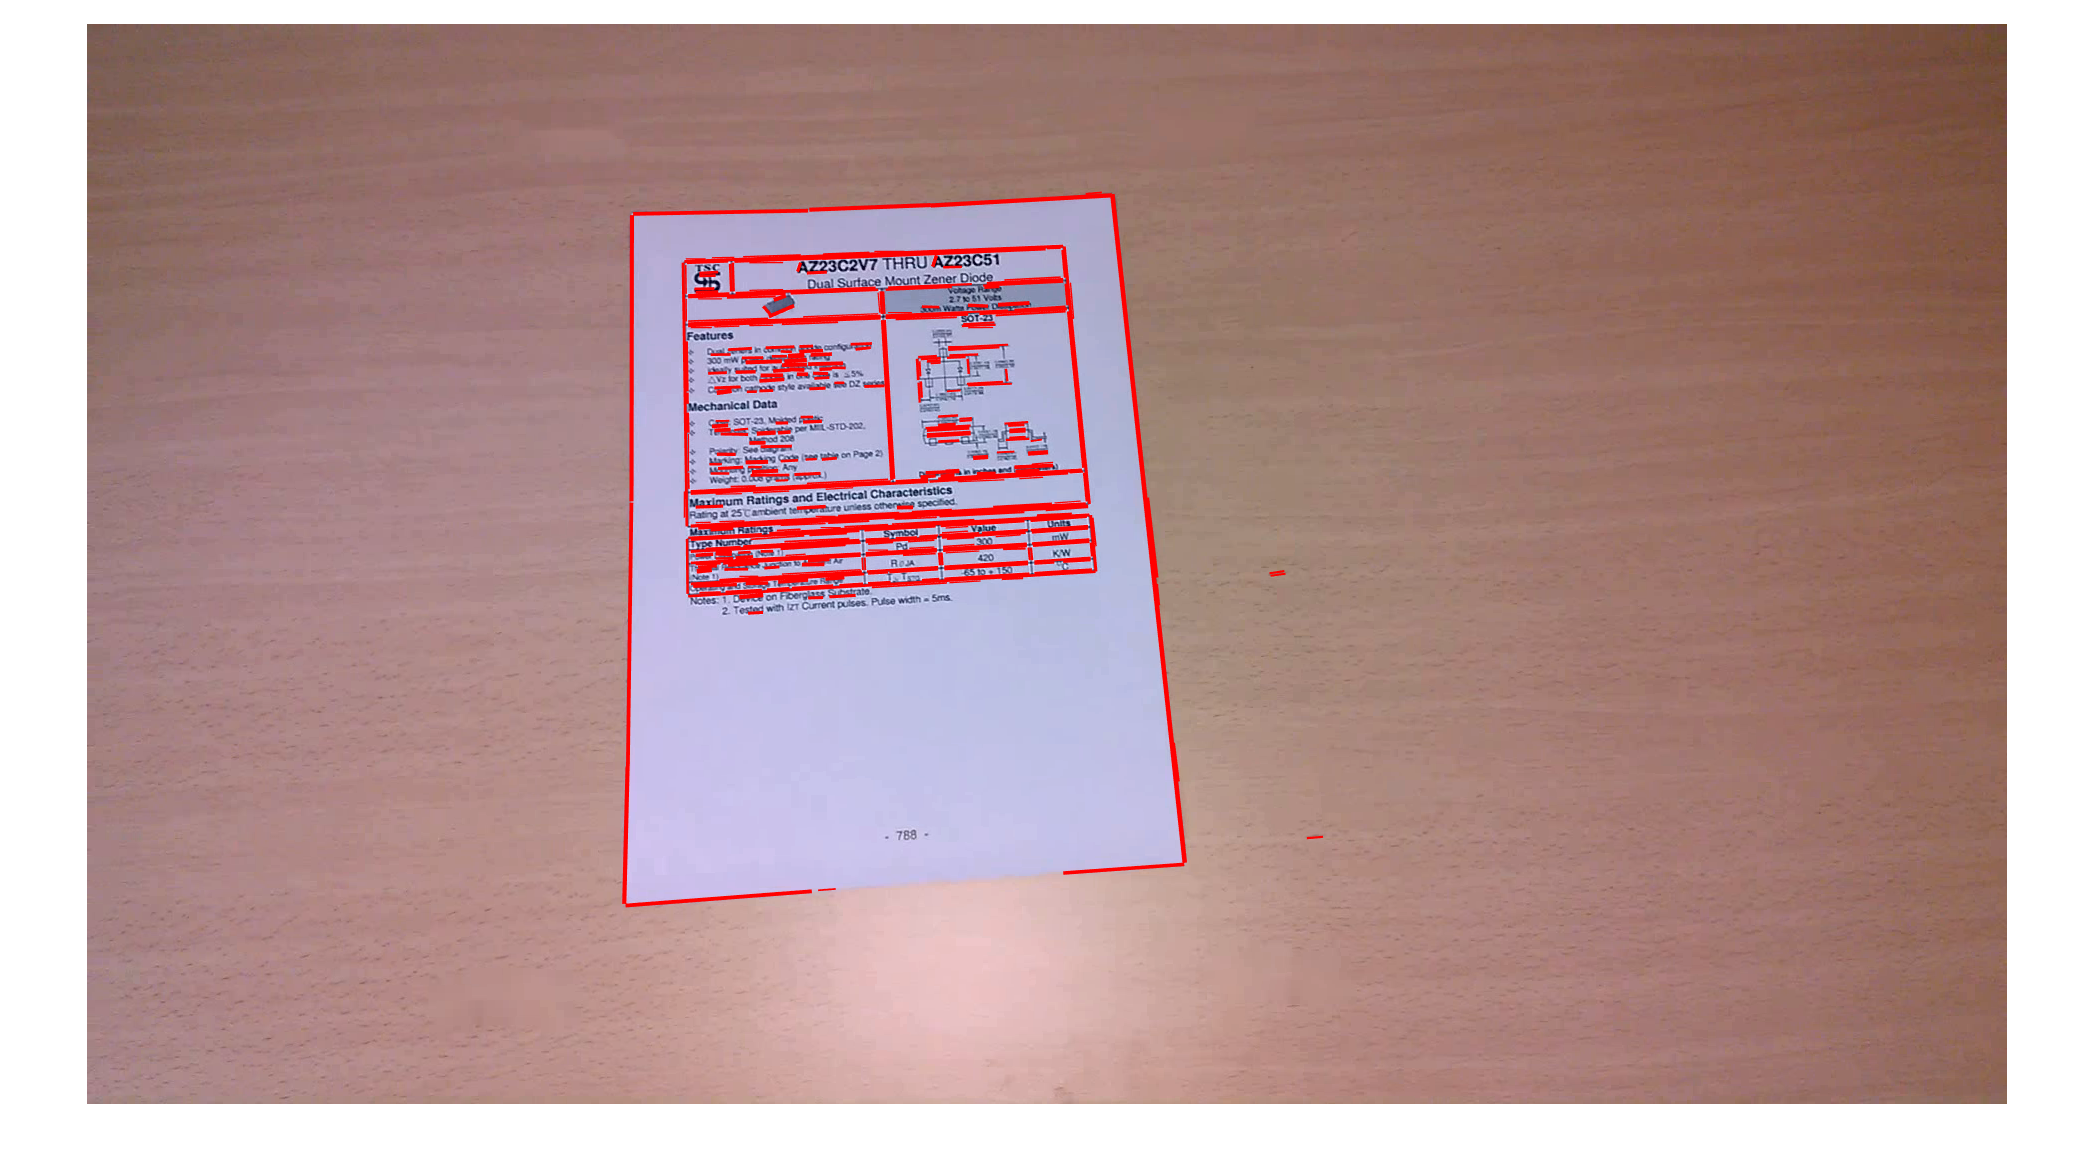
\includegraphics[width=0.7\textwidth]{lsd.png}
\caption{Red lines detected with the LSD algorithm.}
\label{fig:lsd}
\end{figure}

The LSD algorithm detects the essential lines in the image but many lines are very short. Some lines segments represent one line, so we have to merge it.
One of the problems of LSD is that many line segments are detected which are very short
and disconnected, even if they represent one line. For these reasons we
used a technique to merge the detected lines. A naive but inefficient approach
for merging lines would be to iterate the complete enumeration of all line
segment combinations. In contrast, our approach select the first line,
finds all lines sharing a segment with this line and collect them in a list.
Afterwards, all lines in the list are consecutively selected and again all remaining line segments are iterated and if they share an endpoint are added further to the list.
For this reason, each line segment is only processed once and the algorithm yields
therefore a worst case performance of $O(n^2)$. In the best case, if all segments
are a single line, the algorithm has a performance of  $O(n)$.
This step does not only reduce the number of lines and therefore later the number
of candidate bounding boxes but also opens the possibility to search for overlapping
corners and therefore find better fitting bounding boxes.
To further improve the performance and because it is needed during bounding box 
computation anyway, lines are splitted into horizontal and vertical lines based
on their x and y coordinate distance. 
After the line merging, lines are removed based on a minimum length which is 
defined by parameter dependent on the image size. Furthermore, lines are removed which are near the border of the image or which have their starting point on the border of the image as it is assumed that the document is always completely inside the image.\\
The founded set of lines is reduced as follows. 
The result of the post processed set of lines is shown in Figure \ref{fig:redLines}.

\begin{figure}[h]
\centering
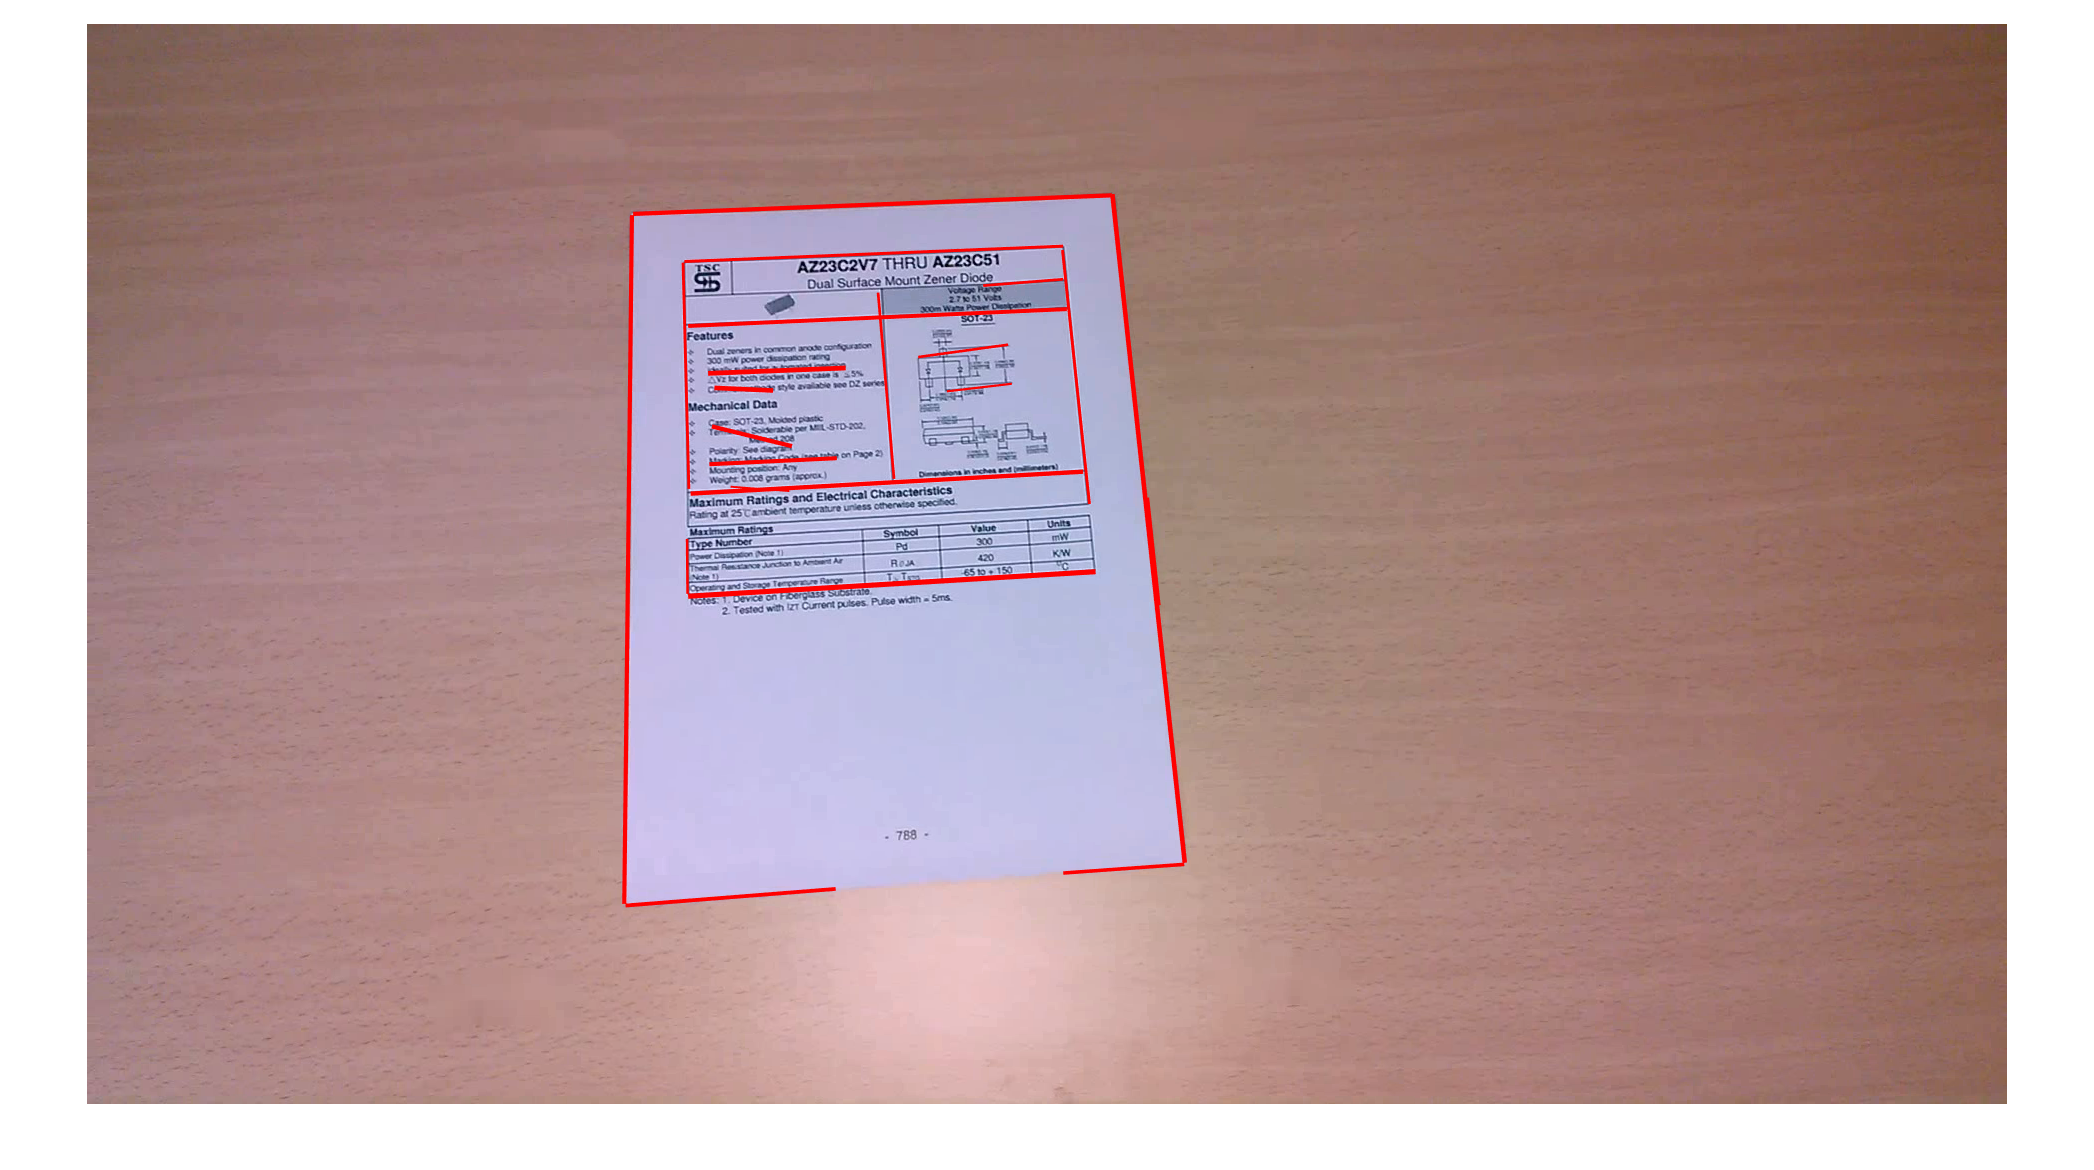
\includegraphics[width=0.7\textwidth]{redLines.png}
\caption{Reduced set of lines.}
\label{fig:redLines}
\end{figure}

\subsection{Bounding Box Calculation}
In the next step, we select two horizontal and two vertical lines and check if both horizontal lines have smaller x coordinates or higher x coordinates as the minimum or maximum x coordinate of the vertical line to check if the line matching make sense. We do the same for vertical lines with the y coordinate. First we select only lines that have at least 3 of 4 similar start, or end points. Then we calculate the bounding boxes of the document.

\subsection{Best Bounding Box Selection}
For every bounding box we calculate the following properties:
\begin{itemize}
\item Area
\begin{itemize}
\item The area is the most important property because we choose the bounding box with the biggest area. Sometimes objects outside of the document are also recognized and would form a bigger area. To counteract this misinterpretation we also check if the area exceeds a certain limit based on the whole image size.
\end{itemize}
\item Length of the horizontal and vertical lines
\begin{itemize}
\item  Even with perspective distortions lines on the opposite of the document
have a similar length.
Hence, we check if the two horizontal lines are equal in length with a little threshold, for vertical lines respectively.
\end{itemize}
\item Aspect ratio
\begin{itemize}
\item Same as for the side lenghts, the aspect ratio should stay similar within in a
certain margin. Therefore, we assume documents in the A4 format in portrait format or horizontal format.
\end{itemize}
\item Inner angles
\begin{itemize}
\item We check if the inner angles are similar to 90 degrees. Due to perspective distortion, which influence angles severely, we accept a high deviation of the angles to achieve suitable results.
\end{itemize}
\end{itemize}

If the bounding box complete the property checks, we choose the bounding box with the greatest area. 
For our previous example, the so found best fitting bounding box is shown in Figure \ref{fig:bb}.
\begin{figure}[h]
\centering
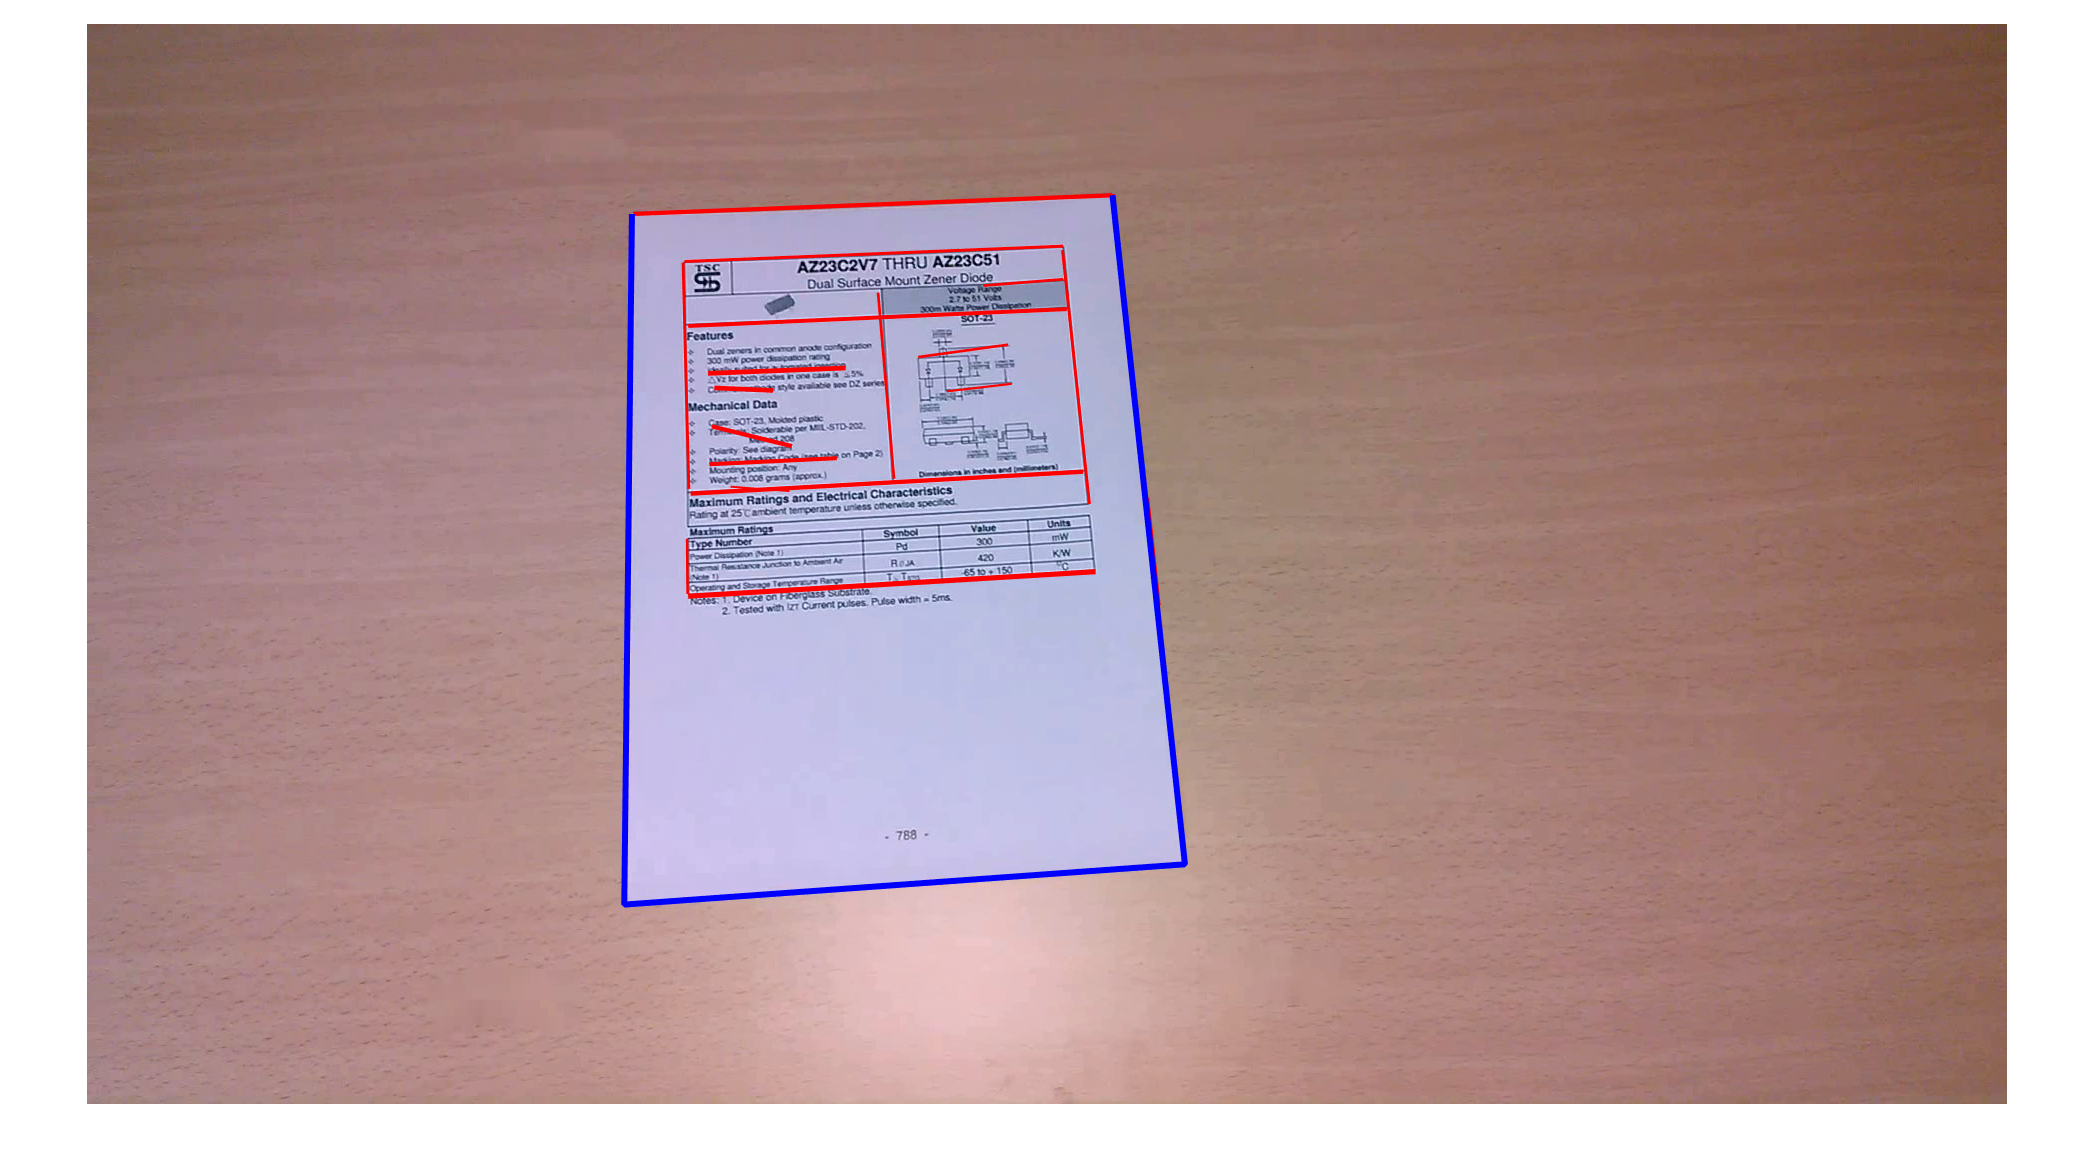
\includegraphics[width=0.7\textwidth]{bb.png}
\caption{Bounding box in blue of the document.}
\label{fig:bb}
\end{figure}

\subsection{Frame Interpolation}
If we get no bounding box from the algorithm or the bounding box is smaller than the average bounding boxes in the complete video we interpolate between frames with areas that have an area greater than the average area of the bounding boxes.

\section{Performance}
One big drawback of the algorithm is the execution time that depends on the number of founded line segments. We calculate for every combination of two horizontal and two vertical lines a bounding box. This is very expense even with a small number of lines due to the permutations. Another problem is that the LSD algorithm takes only an input image path as input. So we have to create an image for every frame and write it out.

\section{Evaluation}
To measure the performance the Jacard index measure \cite{everingham2010pascal} is used. 
The Jacard index is the intersection of the detected bounding box with the ground truth document bounding box divided through the union of the bounding boxes (see equation \ref{eq:1}).
\begin{equation}\label{eq:1}
JI(frame)= \frac{area(G\cap S))}{area(G\cup S))}
\end{equation}

The score for one video is the average of the frame scores, and the overall accuracy of the implemented method is the average of all videos with different backgrounds.

\section{Results}

The computed Jacard indices for the given dataset with our method can be viewed in 
table \ref{tab:results}.

\begin{table*}[]
\centering
\caption{Jacard Index Results}
\label{tax}
\begin{tabular}{l | p{2cm}| p{2cm}| p{2cm}| p{2cm}| p{2cm} }
\hline
& \multicolumn{5}{|c}{\textbf{Background}} \\
\textbf{Document Type} &  \multicolumn{1}{c}{01} & \multicolumn{1}{c}{02} & \multicolumn{1}{c}{03} & \multicolumn{1}{c}{04} &\multicolumn{1}{c}{05} \\ \hline\hline
Datasheet & 0.961804   & 0.933321  &0.956437 &0.338121 &0.419252  \\ 
           &0.969550 & 0.949776  &0.953702 &0.670783 &0.204255  \\ 
           & 0.958112  & 0.926158  &0.954332 &0.460790 &0.407288  \\ 
           & 0.963166  & 0.942556  &0.957530 &0.406976 &0.279959  \\ 
           & 0.956819  & 0.931061  &0.964136 &0.480986 &0.373999  \\ \hline
Letter & 0.966585 & 0.931361  &0.964660 &0.548722 &0.488031  \\    
		& 0.962465 & 0.950924  &0.939243 &0.637083 &0.454185  \\ 
		& 0.962962 & 0.943569  &0.901809 &0.444535 &0.463177  \\ 
		& 0.955535 & 0.945724  &0.939415 &0.690977 &0.405386  \\ 
		& 0.959804 & 0.939154  &0.941210 &0.414960 &0.624913  \\ \hline 
Magazine & 0.961872 & 0.906609  &0.945897 &0.169548 &0.042877  \\   
		& 0.959672 & 0.937086  &0.919084 &0.148990 &0.110548  \\ 
		& 0.922668 & 0.900296  &0.941420 &0.693086 &0.000000  \\ 
		& 0.886081 & 0.863409  &0.915656 &0.389279 &0.552460  \\ 
		& 0.922554 & 0.813186  &0.964260 &0.458704 &0.175053  \\ \hline 	
Paper & 0.956659 & 0.967295  &0.952133 &0.667463 &0.410692  \\   
		& 0.954750 & 0.959377  &0.904080 &0.610046 &0.015565  \\ 
		& 0.943191 & 0.955013  &0.950578 &0.557951 &0.408258  \\ 
		& 0.923238 & 0.947480  &0.971184 &0.643748 &0.447700  \\ 
		& 0.954222 & 0.934069  &0.962020 &0.614676 &0.453615  \\ \hline 	
Patent & 0.944150 & 0.950614  &0.915164 &0.629440 &0.464737  \\   
		& 0.934623 & 0.942731  &0.906549 &0.634424 &0.380177  \\ 
		& 0.939969 & 0.935944  &0.956033 &0.538994 &0.502359  \\ 
		& 0.944970 & 0.918508  &0.897266 &0.226930 &0.358804  \\ 
		& 0.914572 & 0.837318  &0.954834 &0.548980 &0.311188  \\ \hline 
Tax & 0.949686 & 0.902505  &0.944010 &0.342882 &0.490883  \\   
		& 0.940098 & 0.937493  &0.956152 &0.575945 &0.016099  \\ 
		& 0.867588 & 0.938492  &0.933569 &0.466925 &0.062252  \\ 
		& 0.903321 & 0.880571  &0.936461 &0.419935 &0.047539  \\ 
		& 0.951203 & 0.932429  &0.930931 &0.249198 &0.500233  \\ 	\hline \hline 
\textbf{Overall/Background} &0.9431 & 0.9251 & 0.9410 & 0.4894 &0.3290\\ \hline 
\textbf{Overall}&	 0.7255					            
\end{tabular}
\label{tab:results}
\end{table*}

We tried to optimize our approach for the usual case of page detection
with a smartphone. For this reason we optimized our technique for the first three
datasets. 
The fourth background is not really in a natural environment because usually 
the flash light is turned of during video page detection with a smartphone,
though this case is arguable. 
The fifth background does not make any sense as the later for OCR needed
information is anyway overlayed by other stuff. Although, there are more
than one document and it can be argued to decide which document to detect.

Anyway, we tried to improve our solution even for these unrealistic cases.
First we had to tackle that because of missing contrast and overlays not the 
right lines were detected by the LSD.
To overcome this proble, we convert the image in a gray value image. Then we use the canny edge detector with a sigma of 3 to create a binary image of the document. We chose the canny detector because it found most of the edges in the document frames, unlike Sobel or Prewitt. However, there were many distortions on the edges, so we increased the sigma from $\sqrt{2}$ to 4 to smooth the image a bit. The result of the preprocessing steps looks like Figure \ref{fig:pre}.

\begin{figure}[h]
	\centering
	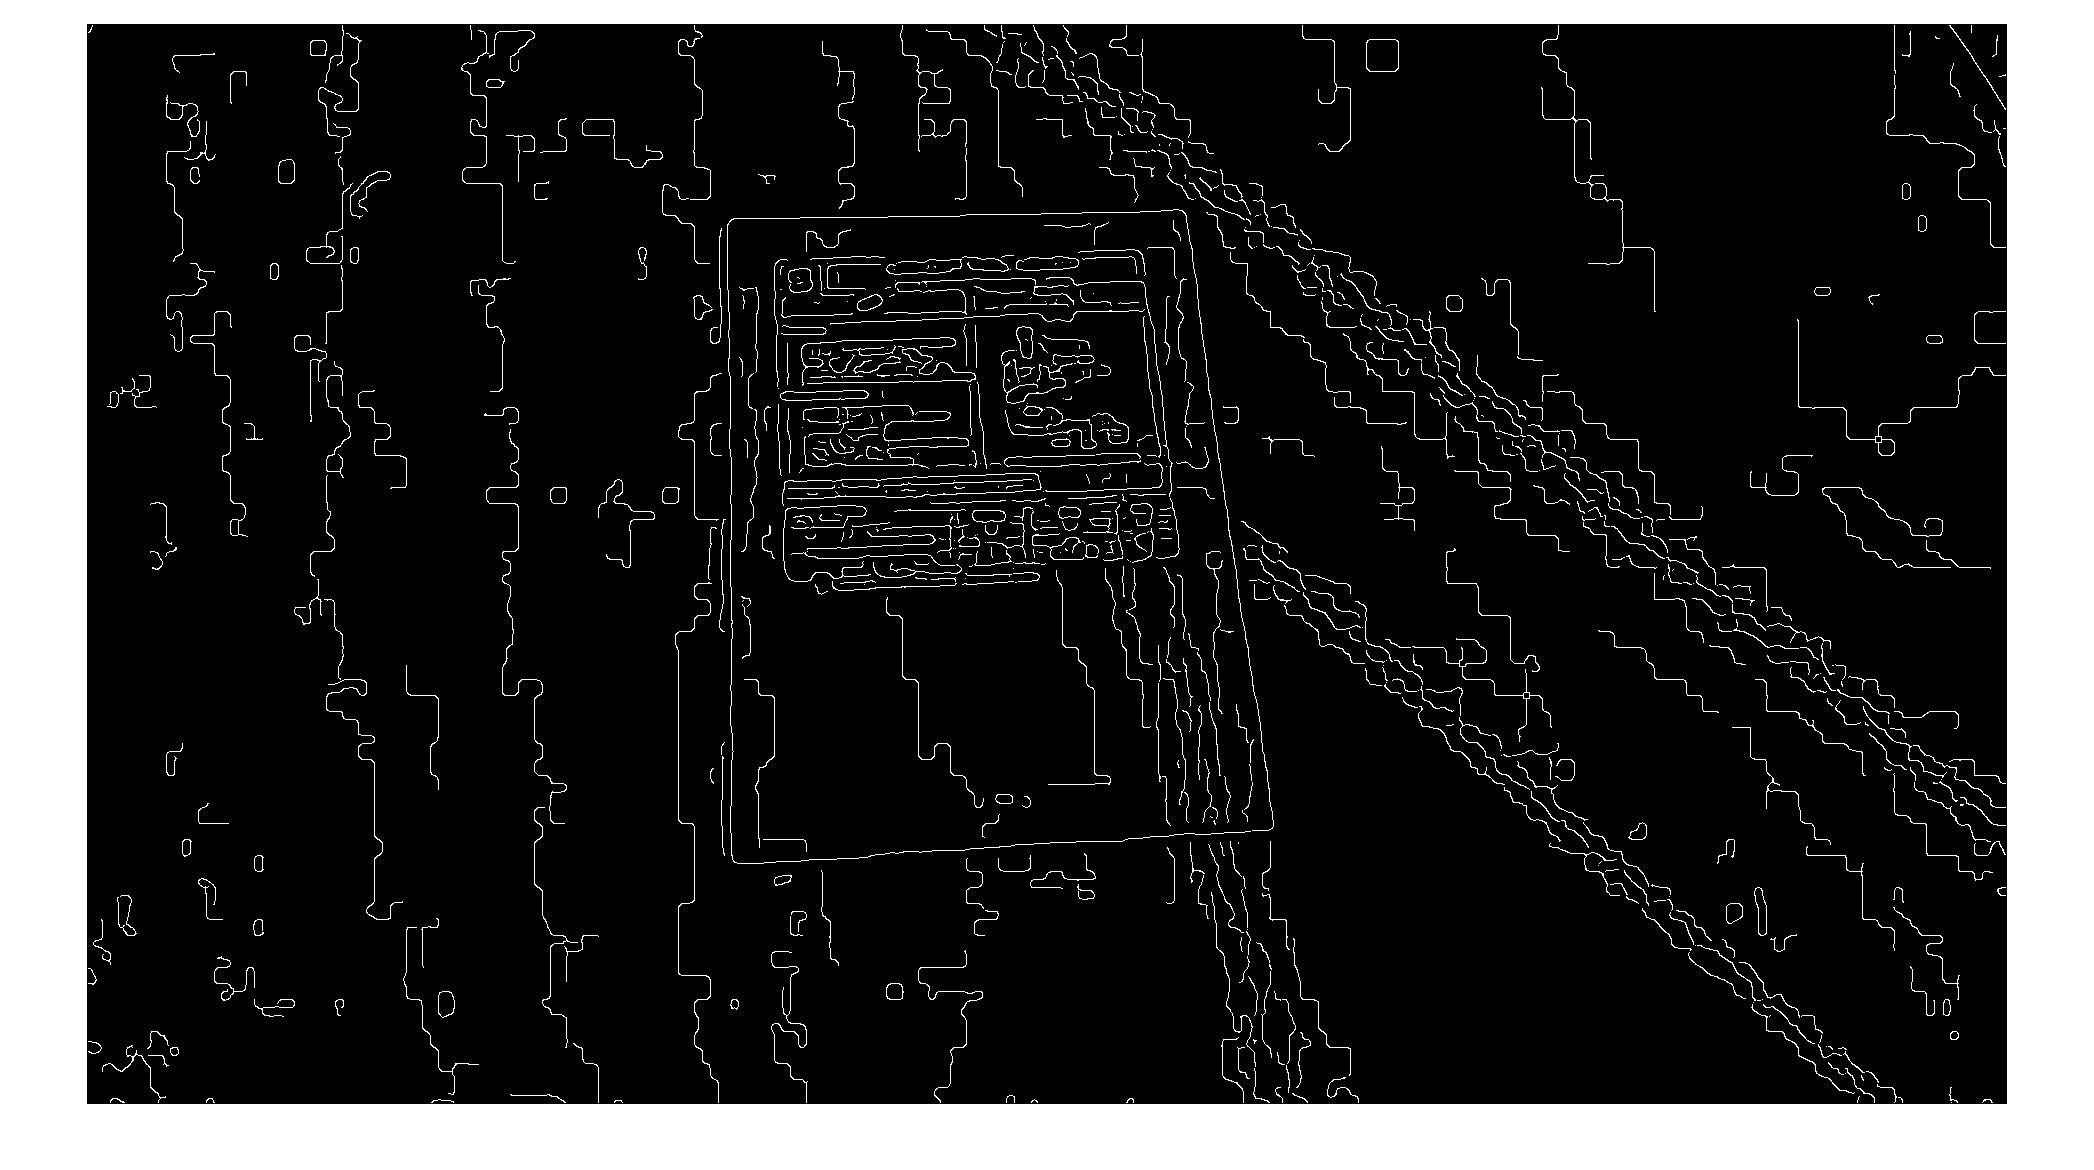
\includegraphics[width=0.7\textwidth]{pre.png}
	\caption{Document frame of the image after the preprocessing step.}
	\label{fig:pre}
\end{figure}

With this preprocessing step the LSD again finds reasonable lines for the datasets
with background four and five. Though, the results only improved to about 60 \%.
For the realistic backgrounds, one, two and three this preprocessing step has a severe impact. Due to the loss of information by converting the image into an edge image,
the important lines get lost for the realistic data sets.
The results are reduced from over 90 \% to about 60 \%. 
For this reason we stayed without the preprocessing step and 
therefore created a method which works quite well for realistic scenarios
(over 90 \%) and fails at unrealistic scenarios, a justifiable trade-off.

It is still to be noted, that for none of the described methods using LSD
a paper could be found. Maybe they changed the method name or someone else
in their research group published the paper with another name
because we searched for the method names and the authors and could not find the papers.
If they really did not publish there methods it is arguable that 
the description is either not complete and some other
criteria for bounding box selection is used or that they optimized
the parameters for the given datasets to achieve these results.

\newpage
\bibliographystyle{plain}
\bibliography{lit}
%% References can be stored in a seperate bib-file (see lit.bib). References, that are cited in the report using \cite are automatically added to the reference list. For more information: http://www.bibtex.org/Using/
%%------------------------------------------------------
\end{document}
